\begin{frame}
	\frametitle{Liguagem: interpretar e classificar}
	Se a elasticidade for, por exemplo, $|\varepsilon_D|=1.3$

	\begin{itemize}
		\setlength{\itemsep}{0.2cm}
		\item \textbf{\underline{Interpreta-se}} dizendo que a quantidade procurada reduz-se 1.3\% se o pre\c co aumentar 1\%, tudo o resto constante.
		\item \textbf{\underline{Classifica-se}} a procura como \underline{\emph{el\'astica}} no ponto onde o valor de $|\varepsilon_D|$ foi calculado.
	\end{itemize}
\end{frame}

\begin{frame}
	\frametitle{Elasticidade Pre\c co-Directa}
	A elasticidade pre\c co-directa da procura tem uma rela\c c\~ao directa com a varia\c c\~ao na despesa de consumo quando se altera um pre\c co.\par
	
	Vejamos o que acontece \`a despesa de consumo quando o pre\c co aumenta \euro 4 em dois cen\'arios diferentes, no exemplo seguinte:
	\begin{itemize}
		\item quando o pre\c co inicialmente \'e \euro 12
		\item quando o pre\c co inicialmente \'e \euro 4
	\end{itemize}
\end{frame}

\begin{frame}
	\frametitle{Elasticidade da Procura}
	$Q_D=100-5P$
	\begin{center}
		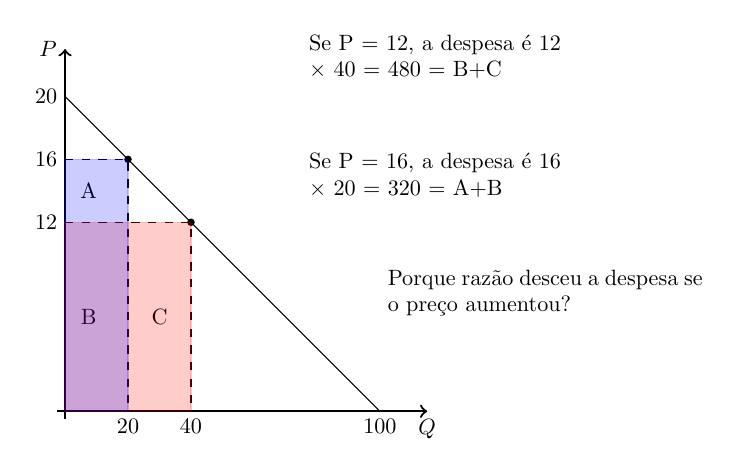
\begin{tikzpicture}[
			scale = 1,
			every node/.style = {scale = 0.8},
			declare function = {d(\x)=4-\x;}
			]

			\draw[->,thick] (-0.1,0) -- (4.6,0)node[below]{$Q$};
			\draw[->,thick] (0,-0.1) -- (0,4.6)node[left]{$P$};

			\draw[domain=0:4,variable=\x] plot (\x,{d(\x)}) node[below]{100};
			\draw(0,{d(0)}) node[left]{20};

			\onslide<2->{
				\draw[dashed](0,2.4)node[left]{12} -- (1.6,2.4)node[circle,fill,inner sep=1.2pt]{} -- (1.6,0)node[below]{40};
				\draw[dashed](0,3.2)node[left]{16} -- (0.8,3.2)node[circle,fill,inner sep=1.2pt]{} -- (0.8,0)node[below]{20};
			}


			\onslide<3->{
				\draw(0.3,2.8)node[]{A};
				\draw(0.3,1.2)node[]{B};
				\draw(1.2,1.2)node[]{C};
			}

			\onslide<4->{
				\draw(3,4.5)node[right]{\parbox{4cm}{Se P = \euro 12, a despesa \'e \euro 12 $\times$ 40 = \euro 480 = B+C}};
			}

			\onslide<5>{
				\draw[opacity=0.2,red,fill] (0,0)--(1.6,0)--(1.6,2.4)--(0,2.4)--(0,0);
			}

			\onslide<6->{
				\draw(3,3)node[right]{\parbox{4cm}{Se P = \euro 16, a despesa \'e \euro 16 $\times$ 20 = \euro 320 = A+B}};	
			}

			\onslide<7>{
				\draw[opacity=0.2,blue,fill] (0,0)--(0.8,0)--(0.8,3.2)--(0,3.2)--(0,0);
			}

			\onslide<8->{
				\draw(4,1.5)node[right]{\parbox{5cm}{Porque raz\~ao desceu a despesa se o pre\c co aumentou?}};	
			}

		\end{tikzpicture}
	\end{center}
\end{frame}


\begin{frame}
	\frametitle{Elasticidade da Procura}
	$Q_D=100-5P$
	\begin{center}
		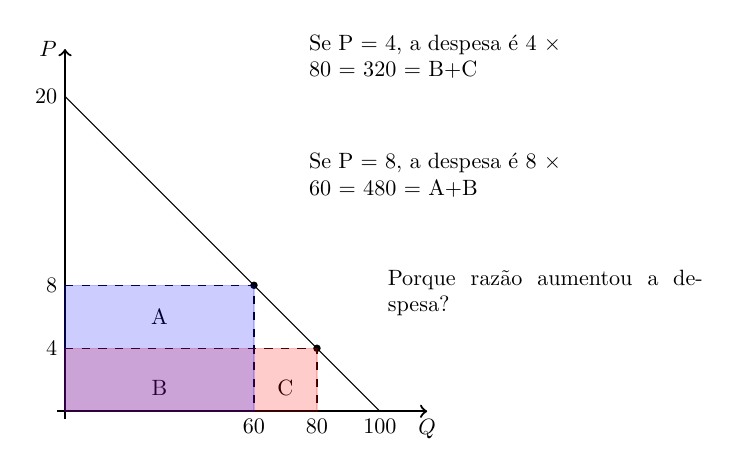
\begin{tikzpicture}[
			scale = 1,
			every node/.style = {scale = 0.8},
			declare function = {d(\x)=4-\x;}
			]

			\draw[->,thick] (-0.1,0) -- (4.6,0)node[below]{$Q$};
			\draw[->,thick] (0,-0.1) -- (0,4.6)node[left]{$P$};

			\draw[domain=0:4,variable=\x] plot (\x,{d(\x)}) node[below]{100};
			\draw(0,{d(0)}) node[left]{20};

			\onslide<2->{
				\draw[dashed](0,0.8)node[left]{4} -- (3.2,0.8)node[circle,fill,inner sep=1.2pt]{} -- (3.2,0)node[below]{80};
				\draw[dashed](0,1.6)node[left]{8} -- (2.4,1.6)node[circle,fill,inner sep=1.2pt]{} -- (2.4,0)node[below]{60};
			}


			\onslide<3->{
				\draw(1.2,1.2)node[]{A};
				\draw(1.2,0.3)node[]{B};
				\draw(2.8,0.3)node[]{C};
			}

			\onslide<4->{
				\draw(3,4.5)node[right]{\parbox{4cm}{Se P = \euro 4, a despesa \'e \euro 4 $\times$ 80 = \euro 320 = B+C}};
			}

			\onslide<5>{
				\draw[opacity=0.2,red,fill] (0,0)--(3.2,0)--(3.2,0.8)--(0,0.8)--(0,0);
			}

			\onslide<6->{
				\draw(3,3)node[right]{\parbox{4cm}{Se P = \euro 8, a despesa \'e \euro 8 $\times$ 60 = \euro 480 = A+B}};	
			}

			\onslide<7>{
				\draw[opacity=0.2,blue,fill] (0,0)--(2.4,0)--(2.4,1.6)--(0,1.6)--(0,0);
			}

			\onslide<8->{
				\draw(4,1.5)node[right]{\parbox{5cm}{Porque raz\~ao aumentou a despesa?}};	
			}

		\end{tikzpicture}
	\end{center}
\end{frame}

\begin{frame}
	\frametitle{Elasticidade e Despesa de Consumo}
	\[Despesa_0=P_0\times Q_0\]
	Seja $\Delta P$ a varia\c c\~ao no pre\c co e $\Delta Q$ a correspondente varia\c c\~ao na quantidade procurada. O valor da despesa total ap\'os a varia\c c\~ao do pre\c co ser\'a
	\[Despesa_1 = \overbrace{(P_0+\Delta P_0)}^{P_1}\times\overbrace{(Q_0+\Delta Q_0)}^{Q_1}\]
	\[=P_0\times Q_0 + P_0\times \Delta Q + \Delta P \times Q_0 + \Delta P \times \Delta Q\]
	Pelo que $\Delta Despesa=Despesa_1-Despesa_0$\[\Delta Despesa =P_0\times \Delta Q + \Delta P \times Q_0 + \Delta P \times \Delta Q\]
\end{frame}

\begin{frame}
	\frametitle{Elasticidade e Despesa de Consumo}
	Notar que se $\Delta P$ \'e pequeno, $\Delta Q$ tamb\'em hai de ser relativamente pequeno (em compara\c c\~ao \`a $Q$),  pelo que $\Delta P\times\Delta Q$ \'e ser\'a muito pequeno, assim podemos dizer que:\[\Delta Despesa \approx P_0\times \Delta Q + \Delta P \times Q_0\]
	Podemos identificar estes dois termos como:

	\begin{itemize}
			\item $\Delta P \times Q_0$ Efeito pre\c co (\'area A do gr\'afico)
			\item $P_0\times \Delta Q$ Efeito quantidade (\'area C do gr\'afico)
	\end{itemize}
\end{frame}

\begin{frame}
\frametitle{Elasticidade e Despesa de Consumo}

	Se a despesa aumenta:

	\begin{align*}
		P_0\times \Delta Q + \Delta P \times Q_0>0 &\Leftrightarrow P_0\times \Delta Q > -\Delta P \times Q_0 \\
		\Leftrightarrow \frac{P\Delta Q}{Q\Delta P}>-1&\Leftrightarrow \frac{\Delta Q}{\Delta P}\frac{P_0}{Q_0}>-1\\ |\varepsilon_D|&<1
	\end{align*}
\end{frame}

\begin{frame}
	\frametitle{Elasticidade e Despesa}
	Ent\~ao:
	\begin{itemize}
		\setlength{\itemsep}{0.5cm}
		\item Numa zona em que a procura \'e el\'astica, $|\varepsilon_D|>1$ um aumento de pre\c co significa uma redu\c c\~ao da despesa (predomina o efeito da redu\c c\~ao da quantidade)
		\item Numa zona em que a procura \'e r\'igida, $|\varepsilon_D|<1$ um aumento de pre\c co significa um aumento da despesa (predomina o efeito do aumento do pre\c co.)
	\end{itemize}
\end{frame}

\begin{frame}
	\frametitle{Elasticidade da Procura}
	$Q_D=100-5P$
	\begin{center}
		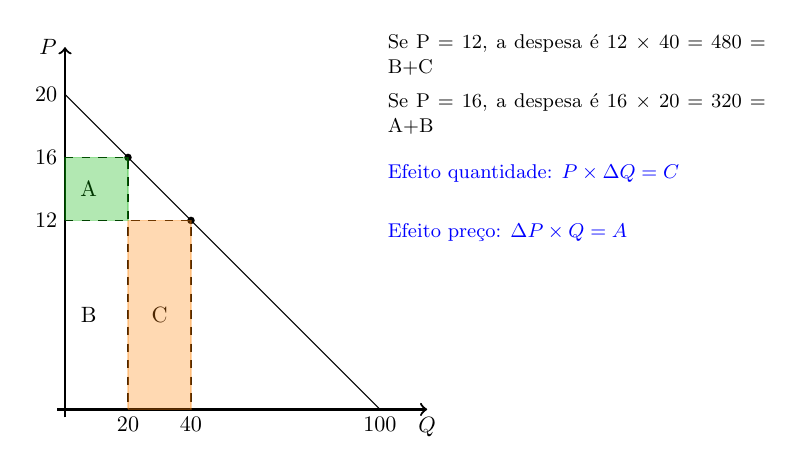
\begin{tikzpicture}[
			scale = 1,
			every node/.style = {scale = 0.8},
			declare function = {d(\x)=4-\x;}
			]

			\draw[->,thick] (-0.1,0) -- (4.6,0)node[below]{$Q$};
			\draw[->,thick] (0,-0.1) -- (0,4.6)node[left]{$P$};

			\draw[domain=0:4,variable=\x] plot (\x,{d(\x)}) node[below]{100};
			\draw(0,{d(0)}) node[left]{20};

			\draw[dashed](0,2.4)node[left]{12} -- (1.6,2.4)node[circle,fill,inner sep=1.2pt]{} -- (1.6,0)node[below]{40};
			\draw[dashed](0,3.2)node[left]{16} -- (0.8,3.2)node[circle,fill,inner sep=1.2pt]{} -- (0.8,0)node[below]{20};

			\draw(0.3,2.8)node[]{A};
			\draw(0.3,1.2)node[]{B};
			\draw(1.2,1.2)node[]{C};

			\draw(4,4.5)node[right]{\parbox{6cm}{\small Se P = \euro 12, a despesa \'e \euro 12 $\times$ 40 = \euro 480 = B+C}};
			\draw(4,3.75)node[right]{\parbox{6cm}{\small Se P = \euro 16, a despesa \'e \euro 16 $\times$ 20 = \euro 320 = A+B}};	

			\onslide<2->{
				\draw(4,3)node[right]{\color{blue}\parbox{6cm}{\small Efeito quantidade: $P\times\Delta Q=C$}};	
			}

			\onslide<3->{
				\draw[opacity=0.3,orange,fill] (0.8,0)--(1.6,0)--(1.6,2.4)--(0.8,2.4)--(0.8,0);
			}

			\onslide<4->{
				\draw(4,2.25)node[right]{\color{blue}\parbox{6cm}{\small Efeito pre\c co: $\Delta P\times Q=A$}};	
			}

			\onslide<5->{
				\draw[opacity=0.3,green!70!black,fill] (0,2.4)--(0.8,2.4)--(0.8,3.2)--(0,3.2)--(0,2.4);
			}

		\end{tikzpicture}
	\end{center}
\end{frame}

\begin{frame}
	\frametitle{Elasticidade da Procura}
	$Q_D=100-5P$
	\begin{center}
		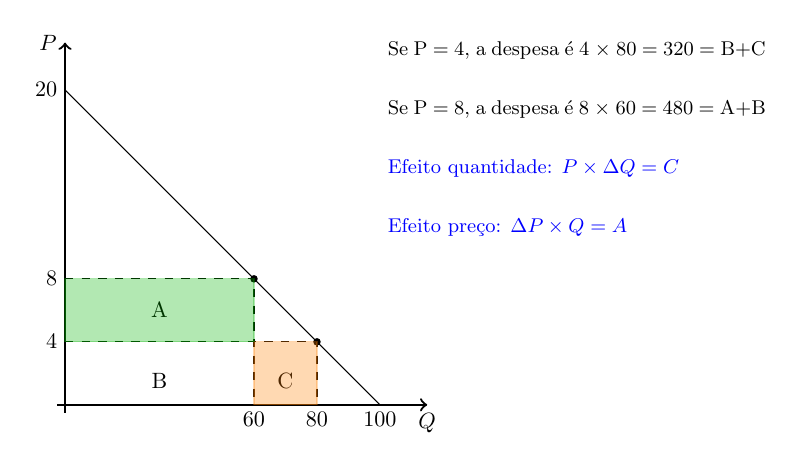
\begin{tikzpicture}[
			scale = 1,
			every node/.style = {scale = 0.8},
			declare function = {d(\x)=4-\x;}
			]

			\draw[->,thick] (-0.1,0) -- (4.6,0)node[below]{$Q$};
			\draw[->,thick] (0,-0.1) -- (0,4.6)node[left]{$P$};

			\draw[domain=0:4,variable=\x] plot (\x,{d(\x)}) node[below]{100};
			\draw(0,{d(0)}) node[left]{20};

			\draw[dashed](0,0.8)node[left]{4} -- (3.2,0.8)node[circle,fill,inner sep=1.2pt]{} -- (3.2,0)node[below]{80};
			\draw[dashed](0,1.6)node[left]{8} -- (2.4,1.6)node[circle,fill,inner sep=1.2pt]{} -- (2.4,0)node[below]{60};

			\draw(1.2,1.2)node[]{A};
			\draw(1.2,0.3)node[]{B};
			\draw(2.8,0.3)node[]{C};

			\draw(4,4.5)node[right]{\parbox{6cm}{\small Se P = \euro 4, a despesa \'e \euro 4 $\times$ 80 = \euro 320 = B+C}};
			\draw(4,3.75)node[right]{\parbox{6cm}{\small Se P = \euro 8, a despesa \'e \euro 8 $\times$ 60 = \euro 480 = A+B}};	

			\onslide<2->{
				\draw(4,3)node[right]{\color{blue}\parbox{6cm}{\small Efeito quantidade: $P\times\Delta Q=C$}};	
			}

			\onslide<3->{
				\draw[opacity=0.3,orange,fill] (2.4,0)--(3.2,0)--(3.2,0.8)--(2.4,0.8)--(2.4,0);
			}

			\onslide<4->{
				\draw(4,2.25)node[right]{\color{blue}\parbox{6cm}{\small Efeito pre\c co: $\Delta P\times Q=A$}};	
			}

			\onslide<5->{
				\draw[opacity=0.3,green!70!black,fill] (0,0.8)--(2.4,0.8)--(2.4,1.6)--(0,1.6)--(0,0.8);
			}

		\end{tikzpicture}
	\end{center}
\end{frame}

\begin{frame}
	\frametitle{Elasticidade da Procura e Despesa:$Q_D=100-5P$}

	\begin{columns}
		\begin{column}{0.6\textwidth}
			\begin{center}
				\begin{tikzpicture}[
					scale = 0.7,
					every node/.style = {scale = 0.5},
					declare function ={
						d(\x) = 4-\x;
					}
					]

					\draw[->,thick] (-0.1,0) -- (5.6,0)node[below]{$Q$};
					\draw[->,thick] (0,-0.1) -- (0,4.6)node[left]{$P$};

					\draw[domain=0:4,variable=\x] plot (\x,{d(\x)})node[below]{$100$};

					\foreach \n/\m in {2.5/87.5,5/75,7.5/62.5,10/50,12.5/37.5,15/25,17.5/12.5,20/0}{
						\draw[dashed](0,{\n/5})node[left]{$\n$} -- ({d(\n/5)},{\n/5}) -- ({d(\n/5)},0)node[below]{$\m$};
					}

					\draw(2,2)node[circle,fill=red,inner sep=2,label=above right:{\(|\varepsilon_D|=1\)}]{};
					\draw[pen colour={red},ultra thick,decorate,decoration={calligraphic brace},yshift=0.1cm,xshift=0.1cm] (2,2) -- (4,0) node[midway,xshift=1cm,yshift=0.1cm]{$|\varepsilon_D|<1$};
					\draw[pen colour={red},ultra thick,decorate,decoration={calligraphic brace},yshift=0.1cm,xshift=0.1cm] (0,4) -- (2,2) node[midway,xshift=0.75cm,yshift=0.25cm]{$|\varepsilon_D|>1$};

					\draw(4,0)node[circle,fill=blue,inner sep=2,label=above right:{\(|\varepsilon_D|=0\)}]{};
					\draw(0,4)node[circle,fill=green,inner sep = 2,label=above right:{\(|\varepsilon_D|=+\infty\)}]{};

					\onslide<2->{

					\draw[->,thick] (-0.1,-4) -- (5.6,-4)node[below]{$Q$};
					\draw[->,thick] (0,-4.1) -- (0,{4.6-6})node[left]{Despesa};

					}

					\onslide<3->{
						\foreach \n/\m/\k/\a in {0/0//a,2.5/87.5/218.75/b,5/75/375/c,7.5/62.5/468.75/d,10/50/500/e,12.5/37.5//f,15/25//g,17.5/12.5//h,20/0/0/i}{

							\draw[dashed](0,{(\n*d(\n/5))/10-4})node[left]{$\k$} -- ({d(\n/5)},{(\n*d(\n/5))/10-4})node[circle,fill,inner sep=1.5,red]{} -- ({d(\n/5)},-4)node[below]{$\m$};
							\draw[dotted]({d(\n/5)},-0.5) -- ({d(\n/5)},{(\n*d(\n/5))/10-4});

							\coordinate (\a) at ({d(\n/5)},{(\n*d(\n/5))/10-4});
						}
					}
					
					\onslide<4>{
						\draw[red,thick] plot [smooth] coordinates {(a) (b) (c) (d) (e) (f) (g) (h) (i)};
					}


				\end{tikzpicture}
			\end{center}
		\end{column}
		\begin{column}{0.375\textwidth}
			{\centering
			\footnotesize
			\begin{tabular}{ccc}
				$P$ & $Q_D$ & $P\times Q_D$\\\hline
				0 & 100 & 0 \\
				2.5 & 87.5 & 218.75 \\
				5 & 75 & 375 \\
				7.5 & 62.5 & 468.75 \\
				10 & 50 & 500 \\
				12.5 & 37.5 & 468.75 \\
				15 & 25 & 375 \\
				17.5 & 12.5 & 218.75 \\
				20 & 0 & 0
			\end{tabular}
		}
		\end{column}
	\end{columns}
\end{frame}

\begin{frame}
	\frametitle{Elasticidade e Despesa de Consumo}
	\begin{columns}
		\begin{column}{0.47\textwidth}
			Generalizando os Resultados:
			\begin{align*}
				Despesa&=RT=P\times Q\\
				P&=\frac{a}{b}-\frac{1}{b}Q\\
				\onslide<2->{
				RT&=\left(\frac{a}{b}-\frac{1}{b}Q\right)\times Q\\
				&=\frac{a}{b}Q-\frac{1}{b}Q^2\\
				}
				\onslide<3->{
				Rmg&=RT'=\frac{a}{b}-\frac{2}{b}Q\\
				Rmg&=0\Leftrightarrow Q=\frac{a}{2}
				}
			\end{align*}
		\end{column}
		\begin{column}{0.47\textwidth}
			\begin{center}
				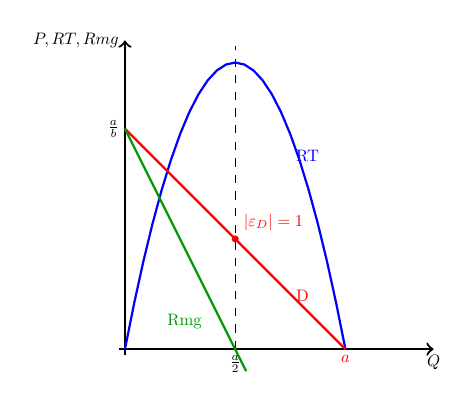
\begin{tikzpicture}[
					scale = 0.7,
					every node/.style = {scale = 0.6},
					declare function = {
						d(\x)=4-\x;
						rt(\x) = 1.3*(4-(\x-2)^2);
						rm(\x) = 4-(2)*\x;
					}]

					\onslide<4->{
						\draw[->,thick] (-0.1,0) -- (5.6,0)node[below]{$Q$};
						\draw[->,thick] (0,-0.1) -- (0,5.6)node[left]{$P,RT,Rmg$};
					}
					
					\onslide<5->{
						\draw[dashed] (2,0)node[below]{$\frac{a}{2}$} -- (2,5.5);
					}

					\onslide<6->{
						\draw[blue,thick,domain=0:4,variable=\x] plot (\x,{rt(\x)});
						\draw[blue] (3,3.5)node[right]{RT};
					}

					\onslide<7->{
						\draw[red,thick,domain=0:4,variable=\x] plot (\x,{d(\x)}) node[below]{$a$};
						\draw[red] (3,0.75)node[above right]{D};	
						\draw[red] (2,2)node[circle,fill,inner sep=1.5,label=above right:{\(|\varepsilon_D|=1\)}]{};
					}

					\onslide<8->{
						\draw[green!60!black,thick,domain=0:2.2,variable=\x] plot (\x,{rm(\x)});
						\draw[green!60!black] (1.5,0.5)node[left]{Rmg};
						\draw(0,{rm(0)}) node[left]{$\frac{a}{b}$};
					}

				\end{tikzpicture}
			\end{center}
		\end{column}
	\end{columns}
\end{frame}

\begin{frame}
	\frametitle{Elasticidade e Despesa de Consumo}
	Formalizando a rela\c c\~ao da receita marginal com a $|\varepsilon_D|$... \par
	Repare-se que $Rmg=\frac{\Delta RT}{\Delta Q}$ \[\Delta RT = \Delta P \times Q + P \Delta Q\] Donde,
	\[Rmg = \frac{\Delta Q\times P + P \times \Delta Q}{\Delta Q} = \frac{\Delta P \times Q}{\Delta Q}+P=P\times\left(\frac{\Delta P\times Q}{\Delta Q\times P}+1\right)=\]
	\[=P\times\left(1+\frac{1}{\varepsilon_D}\right)=P\times\left(1-\frac{1}{|\varepsilon_D|}\right)\]
	Voltaremos a este resultado no cap. 4 (monop\'olio)
\end{frame}

\begin{frame}
	\frametitle{Outras Elasticidades da Procura}
	\begin{itemize}
		\item Elasticidade procura-pre\c co cruzada \[\varepsilon_{x,y}=\frac{\Delta\%Q_x}{\Delta\%P_y}=\frac{\frac{\Delta Q_x}{q_x}}{\frac{\Delta P_y}{P_y}}=\frac{\Delta Q_x}{q_x}\frac{P_y}{\Delta P_y}=\frac{\Delta Q_x}{\Delta P_y}\frac{P_y}{q_x}\]
		\onslide<2->{
		\begin{itemize}
			\item $\varepsilon_{x,y}<0$ caso $X$ e $Y$ sejam bens complementares
			\item $\varepsilon_{x,y}>0$ caso $X$ e $Y$ sejam bens substitutos
			\item $\varepsilon_{x,y}=0$ caso $X$ e $Y$ sejam bens independentes
		\end{itemize}
		}
	\end{itemize}
	\onslide<3->{
	\'E uma ferramenta especialmente importante para determinar os bens que fazem parte do mesmo mercado... quanto mais elevada for $\varepsilon_{x,y}$ maior a influ\^encia m\'utua dos pre\c cos dos bens e, portanto, far\~ao parte do mesmo mercado: iogurtes mimosa e iogurtes danone far\~ao parte do mesmo mercado... mas iogurtes mimosa e ervilhas iglo ser\~ao bens de mercados diferentes, pois nesse caso $\varepsilon_{x,y}=0$}
\end{frame}

\begin{frame}
	\frametitle{Outras Elasticidades da Procura}
	\begin{itemize}
		\item Elasticidade procura-rendimento \[\eta=\frac{\Delta \% Q}{\Delta\% W}=\frac{\frac{\Delta Q}{q}}{\frac{\Delta W}{w}}=\frac{\Delta Q}{\Delta W}\frac{w}{q}\]
	\end{itemize}
	\begin{itemize}
		\item $\eta<0$ para bens inferiores
		\item $\eta>0$ para bens normais
		\onslide<2->{\item $\eta>1$ para bens de luxo}
	\end{itemize}
	Mede a sensibilidade do consumidor face a varia\c c\~oes de rendimento dispon\'ivel para o consumo de um determinado bem.
\end{frame}

\begin{frame}
	\frametitle{Elasticidade Pre\c co da Oferta}
	Calcula-se exactamente da mesma forma do que a elasticidade pre\c co-directa da procura, mas ao longo da curva da oferta...
	\[\varepsilon_s=\frac{\Delta\%Q_S}{\Delta\%P}=\frac{\frac{\Delta Q_S}{Q_S}}{\frac{\Delta P}{P}}=\frac{\Delta Q_S}{\Delta P}\frac{P}{Q_S}\]
	A elasticidade pre\c co da oferta ser\'a \underline{\textbf{sempre positiva}}.

\end{frame}

\begin{frame}
	\frametitle{Elasticidade Pre\c co da Oferta}
	Classifica\c c\~ao da ofeta quanto \`a $\varepsilon_S$
	\begin{itemize}
		\item $\varepsilon_S>1$ $\Rightarrow$ a oferta \'e el\'astica
		\item $\varepsilon_S=1$ $\Rightarrow$ a oferta tem elasticidade unit\'aria
		\item $\varepsilon_S<1$ $\Rightarrow$ a oferta \'e inel\'astica
	\end{itemize}
\end{frame}



\begin{frame}
	\frametitle{Casos extremos}
	\begin{columns}
		\begin{column}{0.47\textwidth}
			\begin{center}
				\begin{tikzpicture}[
					scale = 0.7,
					every node/.style = {scale = 0.7},
					declare function ={
						d(\x) = 4-\x;
					}
					]

					\draw[->,thick] (-0.1,0) -- (5.6,0)node[below]{$Q$};
					\draw[->,thick] (0,-0.1) -- (0,4.6)node[left]{$P$};

					\draw(2,0)node[below]{$Q_0$} -- (2,4)node[midway,xshift=0.25cm]{$S$};

					\onslide<4->{
						\draw(3,1)node[right]{$|\varepsilon_S|=0$};
					}

				\end{tikzpicture}
			\end{center}
			{\scriptsize{
			\onslide<2->{\textbf{A quantidade oferecida \'e independente do pre\c co} (para um intervalo de pre\c cos relevante)}\par
			\onslide<3->{(Ex: qualquer bem para o qual n\~ao seja poss\'ivel aumentar a produ\c c\~ao por aus\^encia de fatores produtivos, e.g.; obras de arte, pe\c cas \'unicas.)}
			}
			}
		\end{column}
		\begin{column}{0.47\textwidth}
			\begin{center}
				\begin{tikzpicture}[
					scale = 0.7,
					every node/.style = {scale = 0.7},
					declare function ={
						d(\x) = 4-\x;
					}
					]

					\draw[->,thick] (-0.1,0) -- (5.6,0)node[below]{$Q$};
					\draw[->,thick] (0,-0.1) -- (0,4.6)node[left]{$P$};

					\draw(0,2)node[left]{$P_0$} -- (4,2)node[midway,yshift=0.25cm]{$S$};

					\onslide<6->{
						\draw(3,1)node[right]{$|\varepsilon_S|=\infty$};
					}

				\end{tikzpicture}
			\end{center}
			
			\onslide<5->{
				\scriptsize{
				Para $P=P_0$ os produtores oferecer\~ao qualquer quantidade... uma expans\~ao da procura n\~ao provocar\'a efeitos inflacionistas... (guardar a informa\c c\~ao para quando se estudar os modelos Keynesianos em Macroeconomia)}
			}
		\end{column}
	\end{columns}
\end{frame}

\begin{frame}
	\frametitle{Factores que influenciam a elasticidade pre\c co da oferta}
	\begin{itemize}
		\item Disponibilidade dos fatores de produ\c c\~ao (incluindo substituibilidade e mobilidade):
		\begin{itemize}
			\item Um quadro de Rembrandt tem uma oferta totalmente, r\'igida, mas a oferta de p\~ao tem uma elasticidade bastante elevada
			\item A oferta de Pizzas ser\'a mais el\'astica do que a oferta de morangos (principalmente se for fora da esta\c c\~ao)
		\end{itemize}
		\item Capacidade produtiva:
		\begin{itemize}
			\item A oferta de transporte a\'ereo \'e inifnitamente el\'astico at\'e se esgotarem os lugares na aeronave, ap\'os o que se torna totalmente r\'igida.
		\end{itemize}
	\end{itemize}
\end{frame}

\begin{frame}
	\frametitle{Factores que influenciam a elasticidade pre\c co da oferta}
	\begin{itemize}
		\item Per\'iodo de tempo: quanto maior o per\'iodo de tempo mais dif\'icil se torna aos produtores o redirecionamento dos factores produtivos e elasticidade da oferta aumenta.
	\end{itemize}
	\begin{columns}
		\begin{column}{0.47\textwidth}
			\begin{center}
				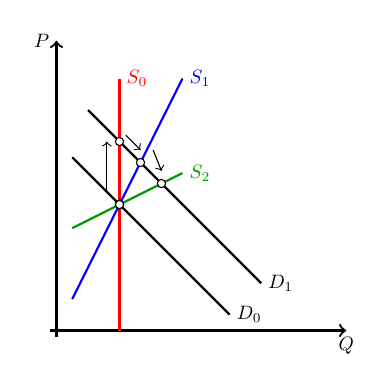
\begin{tikzpicture}[
					scale = 0.8,
					every node/.style = {scale = 0.7},
					declare function = {
						da(\x) = 3-\x;
						db(\x) = 4-\x;
						sa(\x) = 2*\x;
						sb(\x) = 1/2*\x+1.5;
					}
					]

					\draw[->,thick] (-0.1,0) -- (4.6,0)node[below]{$Q$};
					\draw[->,thick] (0,-0.1) -- (0,4.6)node[left]{$P$};

					\onslide<2->{
						\draw[thick,red] (1,0) -- (1,4)node[right]{$S_0$};
					}
					\onslide<3->{
						\draw[thick,domain=0.25:2.75,variable=\x] plot (\x,{da(\x)}) node[right]{$D_0$};
						\draw(1,{da(1)}) node[circle,fill=white,draw,solid,inner sep=1.5]{};

					}
					\onslide<4->{
						\draw[thick,domain=0.5:3.25,variable=\x] plot (\x,{db(\x)}) node[right]{$D_1$};
						\draw(1,{db(1)}) node[circle,fill=white,draw,solid,inner sep=1.5]{};
						\draw[<-] (0.8,{db(1)}) -- (0.8,{da(1)+0.2});
					}

					\onslide<5->{
						\draw[thick,blue,domain=0.25:2,variable=\x] plot (\x,{sa(\x)})node[right]{$S_1$};
						\draw({4/3},{sa(4/3)}) node[circle,fill=white,draw,solid,inner sep=1.5]{};
						\draw(1,{da(1)}) node[circle,fill=white,draw,solid,inner sep=1.5]{};
						\draw[->] ({1+0.1},{db(1)+0.1}) -- ({4/3},{sa(4/3)+0.2});
					}

					\onslide<6->{
						\draw[thick,green!60!black,domain=0.25:2,variable=\x] plot (\x,{sb(\x)})node[right]{$S_2$};
						\draw({5/3},{sb(5/3)}) node[circle,fill=white,draw,solid,inner sep=1.5]{};
						\draw(1,{da(1)}) node[circle,fill=white,draw,solid,inner sep=1.5]{};
						\draw[->] ({4/3+0.2},{sa(4/3)+0.2}) -- ({5/3},{sb(5/3)+0.2});
					}

				\end{tikzpicture}
			\end{center}
		\end{column}
		\begin{column}{0.47\textwidth}
			{\scriptsize
			A curto prazo, uma expans\~ao da procura de viagens para um destino em que os avi\~oes est\~ao sempre cheios s\'o ter\'a um efeito de aumento de pre\c cos: apenas os consumidores com maior disponibilidade a pagar poder\~ao viajar... ao longo prazo, podem planear-se mais voos para satisfazer a procura, podendo o pre\c co descer.
			}
		\end{column}
	\end{columns}
\end{frame}

\begin{frame}
	\frametitle{Quadro resumo Elasticidades}
	\begin{center}
		\begin{tabular}{ccc}
		\rowcolor{red!20!white} \textbf{Elasticidade} & \textbf{Valor} & \textbf{Conclus\~ao}\\ \hline
		\rowcolor{red!10!white}& $>1$ & Procura \'e el\'astica \\
		\rowcolor{red!10!white}& $= 1$ & Procura tem elasticidade unit\'aria \\
		\rowcolor{red!10!white}\multirow{-3}{*}{$|\varepsilon_D|$}& $< 1$ & Procura \'e inel\'astica \\ \hline
		\rowcolor{red!20!white}& $> 0$ & Bens substitutos\\
		\rowcolor{red!20!white}& $= 0$ & Bens independentes \\
		\rowcolor{red!20!white}\multirow{-3}{*}{$|\varepsilon_{x,y}|$}& $> 0$ & Bens complementares \\ \hline
		\rowcolor{red!10!white}& $< 0$ & Bem inferior \\
		\rowcolor{red!10!white}& $0<\eta<1$ & Bem normal \\
		\rowcolor{red!10!white}\multirow{-3}{*}{$\eta$}& $> 1$ & Bem de luxo \\\hline
		\rowcolor{red!20!white}& $> 1$ & Oferta \'e el\'astica\\
		\rowcolor{red!20!white}& $= 1$ & Oferta tem elasticidade unit\'aria \\
		\rowcolor{red!20!white}\multirow{-3}{*}{$\varepsilon_S$}& $< 1$ & Oferta \'e inel\'astica
		\end{tabular}
	\end{center}
\end{frame}